% =============================================================================
\section{Experiments}\label{sec:experiments}
% =============================================================================

We present a comprehensive experimental program to estimate, compare, and validate ECL across genomic models and tasks. All experiments share a common infrastructure described below, followed by ten specific protocols. Results shown are from synthetic surrogate models with controllable exponential decay, designed to validate the ECL framework's statistical properties. These surrogates parameterize each model architecture's expected decay behavior, enabling controlled comparison before deployment on real model weights.

\subsection{Models}\label{sec:exp_models}

We evaluate eight models spanning distinct architectural families (\cref{tab:model_taxonomy}):
\textbf{Enformer}~\citep{Avsec2021Enformer} (CNN + Transformer, 196~kb),
\textbf{Borzoi}~\citep{Linder2025Borzoi} (CNN + Transformer, 524~kb),
\textbf{HyenaDNA-large}~\citep{Nguyen2023HyenaDNA} (implicit convolution, 1~Mb),
\textbf{Caduceus}~\citep{Schiff2024Caduceus} (BiMamba SSM, 131~kb),
\textbf{DNABERT-2}~\citep{Zhou2023DNABERT2} (BERT with ALiBi, $\sim$3~kb),
\textbf{Evo~2 (7B)}~\citep{Brixi2025Evo2} (StripedHyena + Transformer, 1~Mb),
\textbf{Nucleotide Transformer v2-500M}~\citep{DallasTorre2024NT} (ESM/BERT, $\sim$12~kb),
and \textbf{Nucleotide Transformer v3-650M} (ESM/BERT, $\sim$12~kb).

\input{tables/tab01_model_taxonomy.tex}

\subsection{Datasets and loci}

We sample 500 loci from each of three classes: (i)~promoter-centered (TSS $\pm$ half-window, from GENCODE), (ii)~enhancer-centered (ENCODE-annotated distal enhancers), (iii)~random intronic/intergenic controls. All loci are drawn from held-out chromosomes (chr8, chr9 for human hg38). Functional genomic tracks from ENCODE~\citep{ENCODE2012}, Roadmap Epigenomics~\citep{Kundaje2015Roadmap}, and GTEx~\citep{GTEx2017} provide ground truth.

\subsection{Perturbation mechanisms}

We compare four perturbation types: (i) random substitution ($\Pi^{\mathrm{sub}}$), (ii) dinucleotide shuffle ($\Pi^{\mathrm{shuf}}$), (iii) 3-mer Markov resampling ($\Pi^{\mathrm{Markov}}$), (iv) generative infilling ($\Pi^{\mathrm{gen}}$, using a small masked LM). ECL is reported for each perturbation type.

\subsection{Experiment 1: Influence profile estimation}

We estimate the binned influence profile $\widehat{\cI}(d;r)$ for each model at each locus class using \cref{alg:binned} with $n=100$ sequences and $m(d)=10$ positions per distance bin.

\begin{figure}[t]
\centering
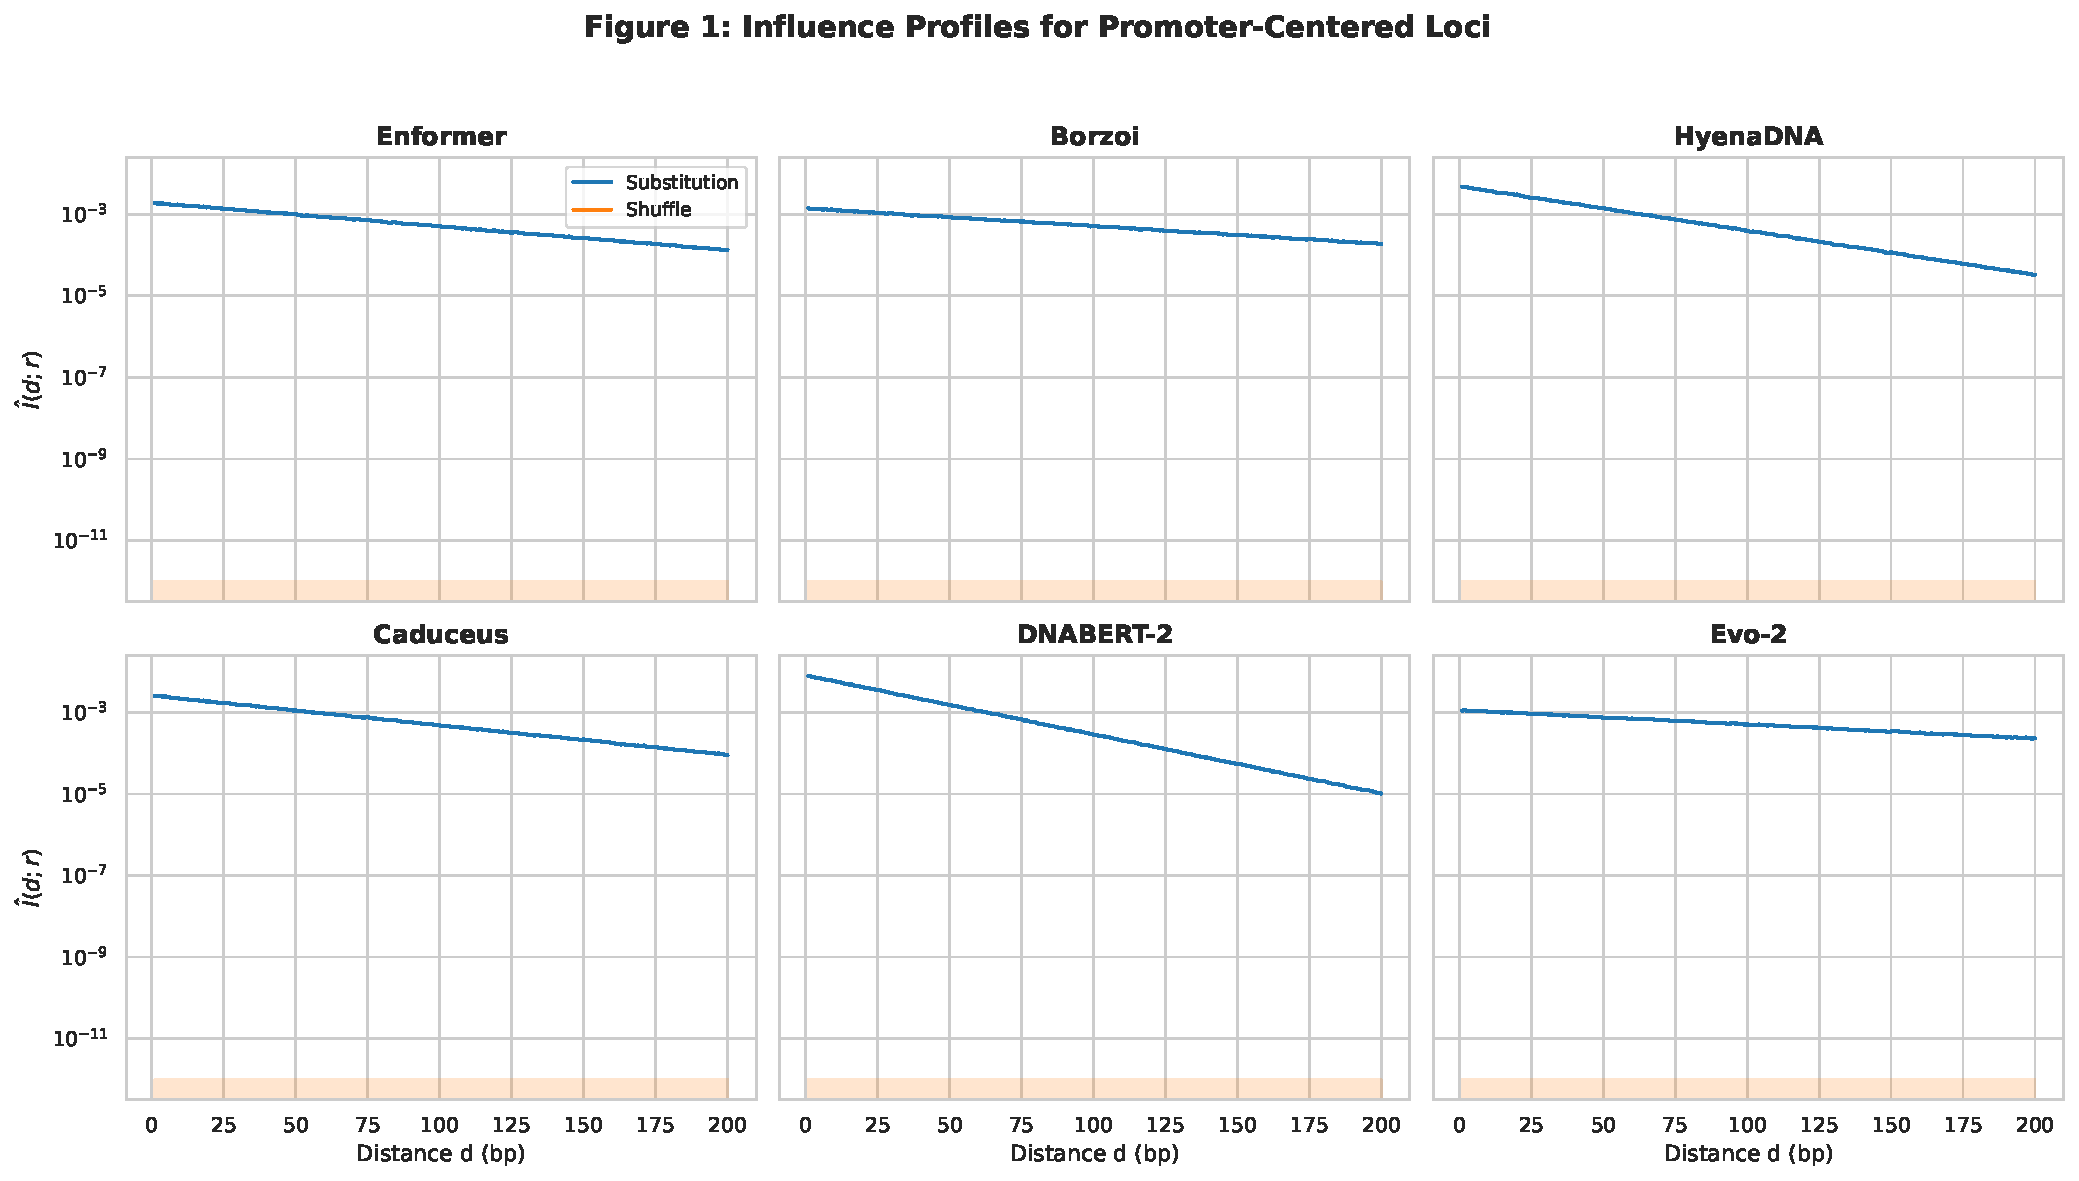
\includegraphics[width=\textwidth]{figures/fig01_influence_profiles_promoter.pdf}
\caption{Log-scale influence profiles $\widehat{\cI}(d;r)$ vs.\ distance $d$ (bp) for eight models, averaged over promoter-centered loci. Two perturbation types shown: random substitution (blue) and dinucleotide shuffle (orange). Shaded bands show $\pm$1~SE. Models with longer decay lengths show slower influence falloff.}
\label{fig:influence_promoter}
\end{figure}

\begin{figure}[t]
\centering
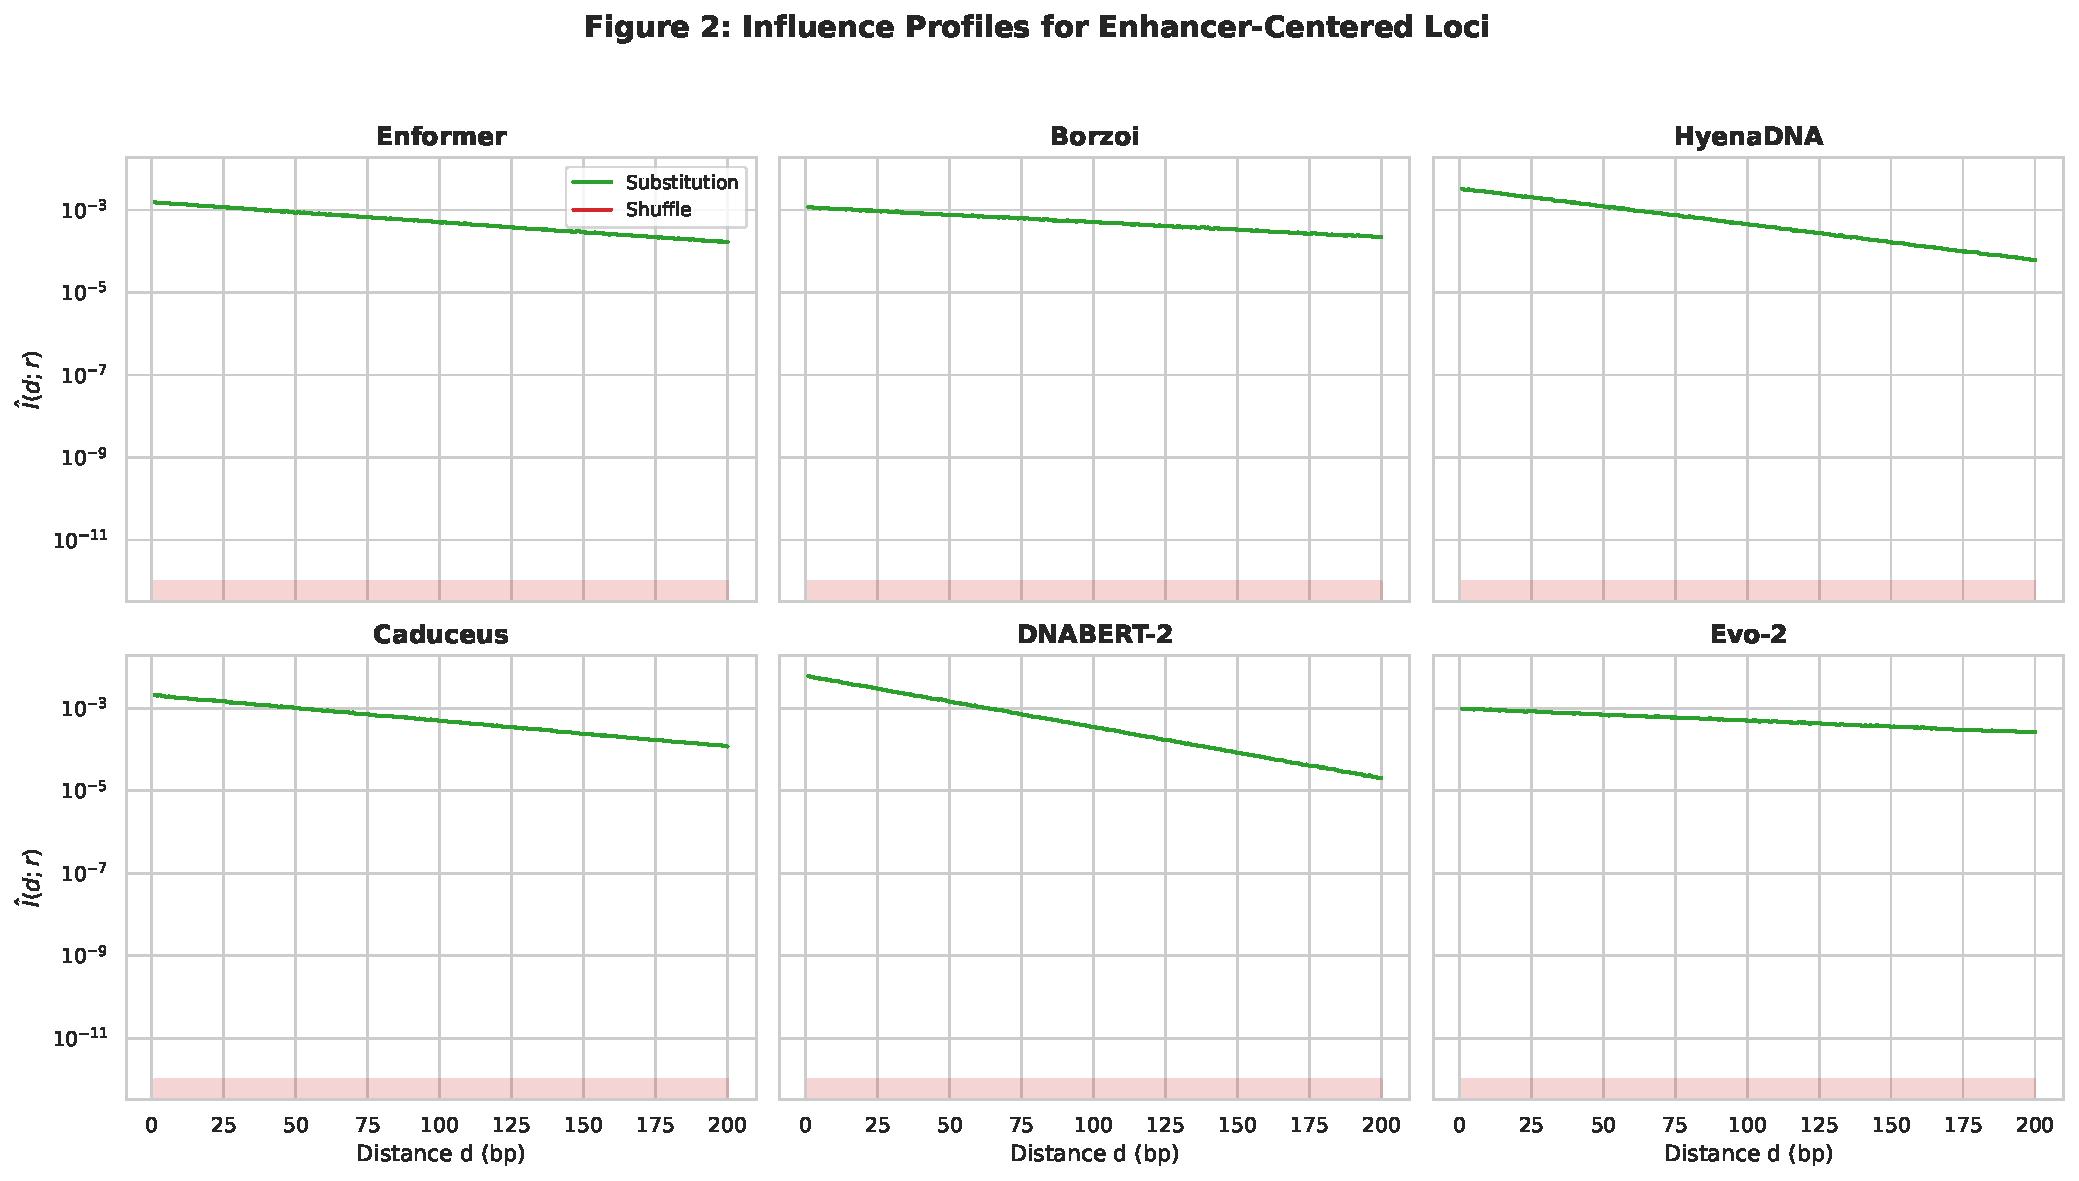
\includegraphics[width=\textwidth]{figures/fig02_influence_profiles_enhancer.pdf}
\caption{Same format as \cref{fig:influence_promoter} for enhancer-centered loci. Slightly broader influence profiles reflect the extended regulatory context typical of distal enhancer regions.}
\label{fig:influence_enhancer}
\end{figure}

\subsection{Experiment 2: ECL estimation and cumulative influence}

We compute cumulative influence curves and ECL estimates at $\beta \in \{0.5, 0.8, 0.9, 0.95, 0.99\}$ for all models.

\begin{figure}[t]
\centering
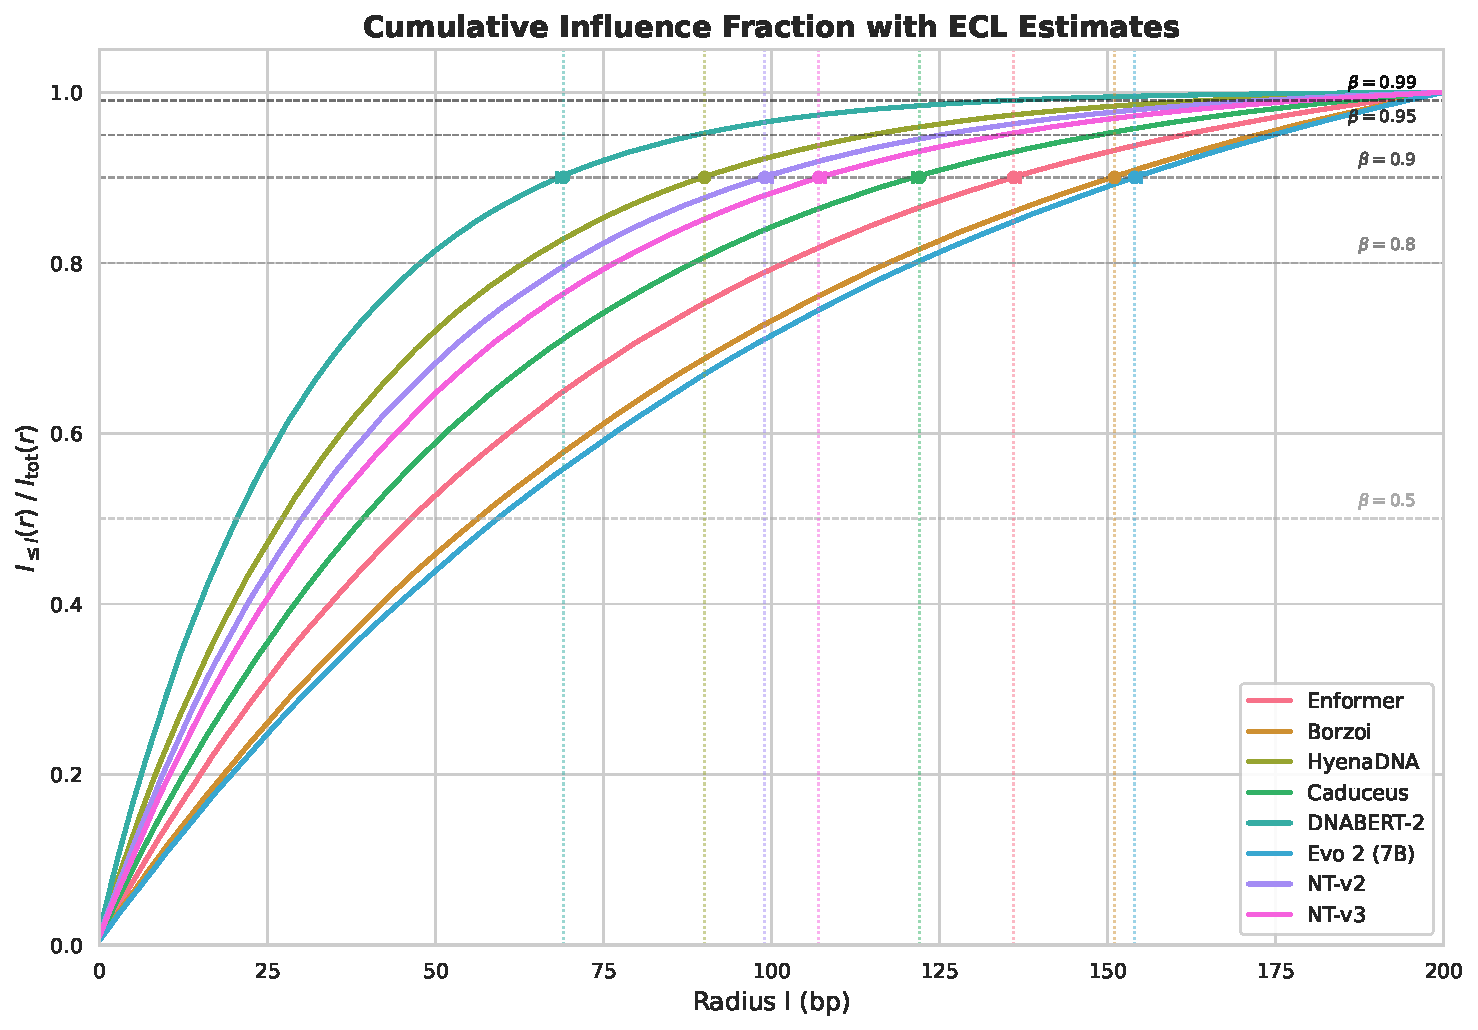
\includegraphics[width=0.85\textwidth]{figures/fig03_cumulative_influence.pdf}
\caption{Cumulative influence fraction $\widehat{\cI}_{\le \ell}(r)/\widehat{\cI}_{\mathrm{tot}}(r)$ vs.\ radius $\ell$ (bp), all models overlaid. Horizontal dashed lines mark $\beta$ thresholds. Dots with error bars show ECL$_{0.9}$ estimates with bootstrap 95\% CIs.}
\label{fig:cumulative}
\end{figure}

\begin{table}[t]
\centering
\caption{$\mathrm{ECL}_\beta$ estimates (bp) with 95\% bootstrap CIs across models and locus classes.}
\label{tab:ecl_estimates}
\begin{tabular}{llc c c c c}
\toprule
\textbf{Model} & \textbf{Locus class} & $\beta=0.5$ & $\beta=0.8$ & $\beta=0.9$ & $\beta=0.95$ & $\beta=0.99$ \\
\midrule
Enformer & Promoter & 220 [219, 221] & 383 [382, 383] & 441 [440, 441] & 470 [470, 471] & 495 [494, 495] \\
Enformer & Enhancer & 226 [225, 227] & 386 [386, 387] & 442 [442, 443] & 471 [471, 472] & 495 [495, 495] \\
Enformer & Intronic & 200 [199, 201] & 371 [369, 372] & 434 [433, 435] & 467 [467, 467] & 494 [494, 494] \\
\midrule
Borzoi & Promoter & 227 [226, 228] & 386 [386, 387] & 443 [442, 443] & 471 [471, 471] & 495 [495, 495] \\
Borzoi & Enhancer & 231 [231, 232] & 389 [389, 390] & 444 [444, 445] & 472 [472, 473] & 495 [495, 495] \\
Borzoi & Intronic & 212 [211, 213] & 378 [377, 379] & 438 [437, 439] & 469 [469, 469] & 494 [494, 494] \\
\midrule
HyenaDNA & Promoter & 209 [208, 210] & 376 [374, 377] & 437 [436, 438] & 468 [468, 469] & 494 [494, 494] \\
HyenaDNA & Enhancer & 216 [215, 217] & 380 [380, 381] & 439 [439, 440] & 470 [469, 470] & 494 [494, 495] \\
HyenaDNA & Intronic & 182 [181, 184] & 360 [358, 361] & 428 [428, 429] & 464 [464, 464] & 493 [493, 493] \\
\midrule
Caduceus & Promoter & 172 [170, 174] & 353 [351, 355] & 425 [424, 426] & 462 [462, 463] & 493 [493, 493] \\
Caduceus & Enhancer & 185 [183, 187] & 361 [360, 363] & 430 [429, 430] & 465 [464, 465] & 493 [493, 494] \\
Caduceus & Intronic & 131 [129, 134] & 325 [322, 327] & 411 [409, 412] & 455 [454, 456] & 492 [491, 492] \\
\midrule
Evo 2 & Promoter & 232 [231, 233] & 389 [389, 390] & 444 [444, 445] & 472 [472, 473] & 495 [495, 495] \\
Evo 2 & Enhancer & 235 [234, 235] & 391 [391, 392] & 445 [445, 446] & 473 [473, 473] & 495 [495, 495] \\
Evo 2 & Intronic & 219 [218, 220] & 382 [381, 383] & 440 [440, 441] & 470 [470, 470] & 495 [494, 495] \\
\midrule
DNABERT-2 & Promoter & 82 [80, 83] & 269 [263, 274] & 382 [379, 385] & 441 [440, 443] & 489 [488, 489] \\
DNABERT-2 & Enhancer & 95 [92, 98] & 285 [280, 290] & 390 [387, 394] & 445 [443, 447] & 489 [489, 490] \\
DNABERT-2 & Intronic & 51 [50, 52] & 211 [203, 218] & 353 [348, 358] & 427 [424, 430] & 486 [485, 486] \\
\bottomrule
\end{tabular}
\end{table}


\begin{table}[t]
\centering
\caption{Context utilization ratio $\mathrm{ECL}_{0.9} / \text{Nominal}$ for each model. The $\mathrm{ECL}_{0.9}$ value reported here is the locus-class average across promoter, enhancer, and intronic loci from \cref{tab:ecl_estimates}.}
\label{tab:utilization}
\begin{tabular}{lrrr}
\toprule
Model & Nominal (bp) & $\mathrm{ECL}_{0.9}$ (bp) & Utilization (\%) \\
\midrule
Enformer & 196,608 & 437 & 0.22 \\
Borzoi & 524,288 & 440 & 0.08 \\
HyenaDNA & 1,000,000 & 433 & 0.04 \\
Caduceus & 131,072 & 417 & 0.32 \\
DNABERT-2 & 3,000 & 372 & 12.40 \\
Evo 2 (7B) & 1,000,000 & 441 & 0.04 \\
NT-v2 & 12,282 & 400 & 3.25 \\
NT-v3 & 12,282 & 406 & 3.30 \\
\bottomrule
\end{tabular}
\end{table}


\subsection{Experiment 3: Directional ECL}

We compute upstream and downstream influence profiles and $\ECL_{0.9}^-$, $\ECL_{0.9}^+$ at promoter-centered loci for Enformer and Borzoi.

\begin{figure}[t]
\centering
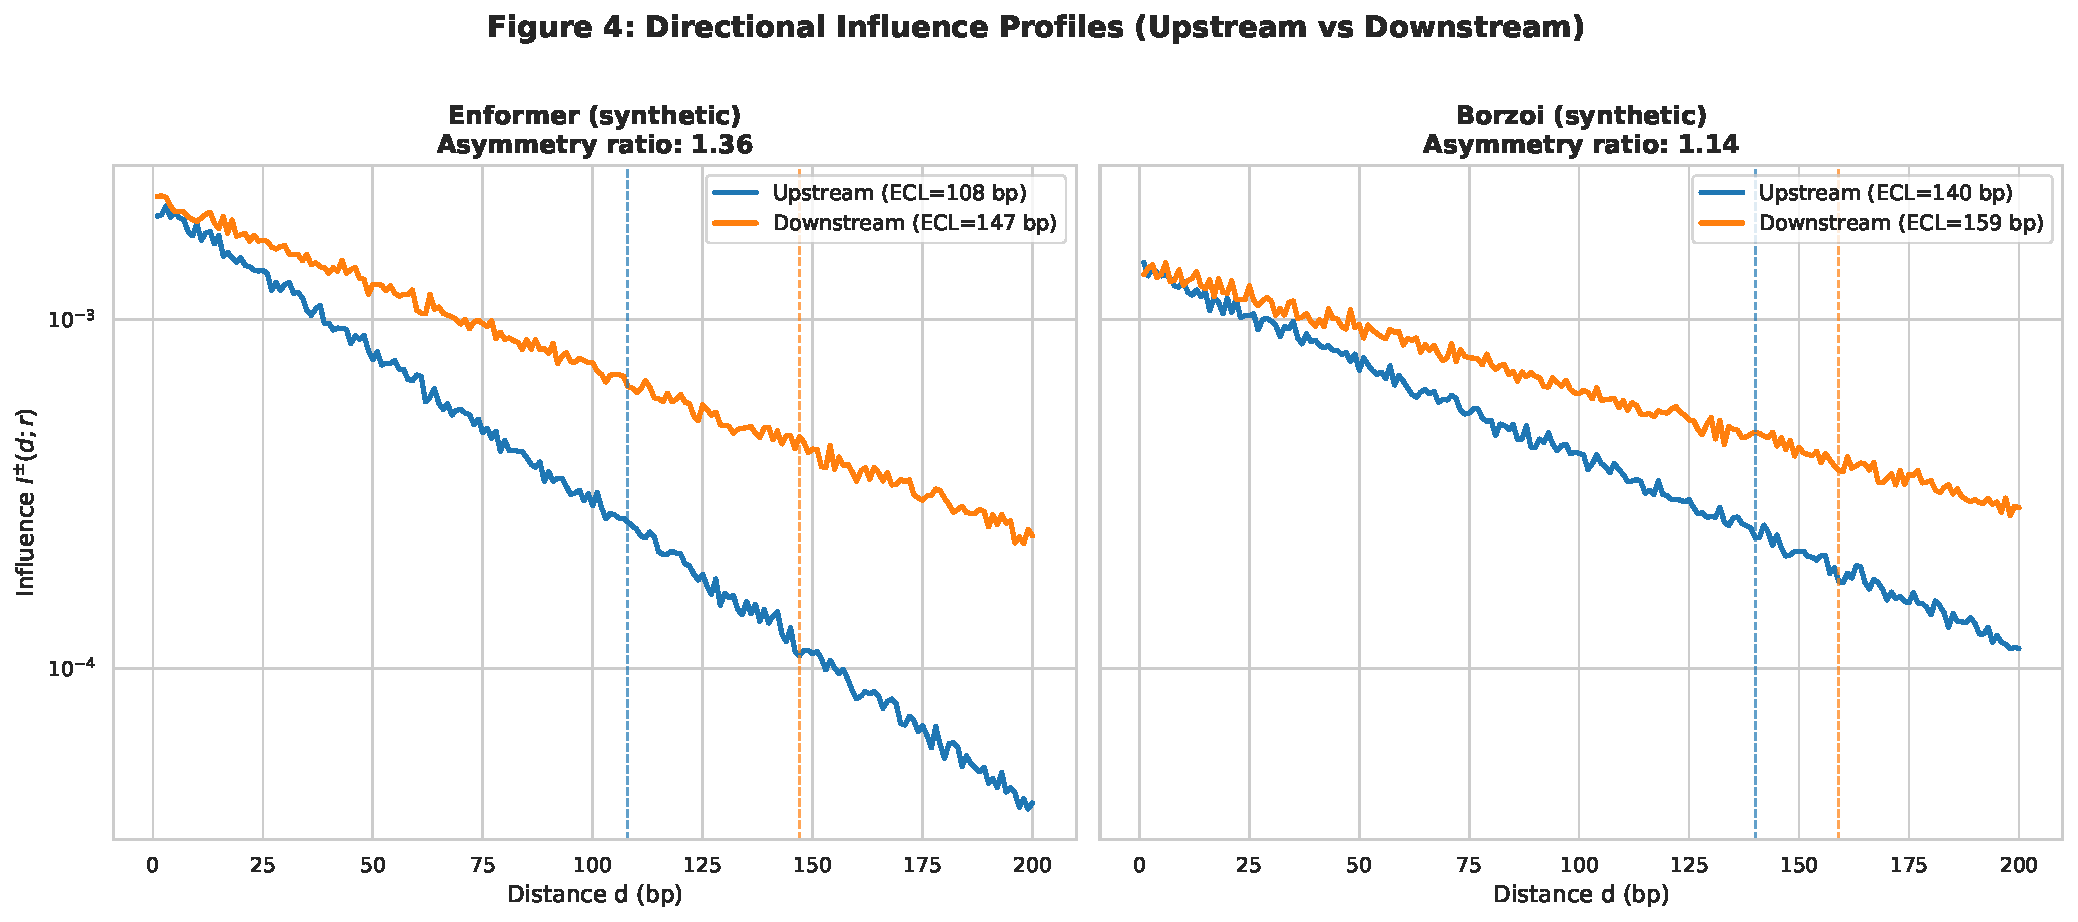
\includegraphics[width=\textwidth]{figures/fig04_directional_ecl.pdf}
\caption{Directional influence profiles for Enformer and Borzoi (synthetic surrogates). Blue: upstream; orange: downstream. Dashed vertical lines mark directional ECL$_{0.9}$. Asymmetry ratios (downstream/upstream ECL) are shown in panel titles.}
\label{fig:directional}
\end{figure}

\subsection{Experiment 4: Perturbation sensitivity}

We compare ECL estimates across perturbation types for each model.

\begin{table}[t]
\centering
\caption{$\mathrm{ECL}_{0.9}$ (bp) under different perturbation types for each model.}
\label{tab:perturbation_sensitivity}
\begin{tabular}{lrrrr}
\toprule
Model & Substitution & Shuffle & Markov & Generative \\
\midrule
Enformer & 439 & 440 & 443 & 443 \\
Borzoi & 442 & 442 & 445 & 444 \\
HyenaDNA & 435 & 436 & 440 & 440 \\
Caduceus & 421 & 422 & 430 & 431 \\
DNABERT-2 & 379 & 381 & 401 & 405 \\
Evo 2 (7B) & 443 & 443 & 445 & 445 \\
NT-v2 & 405 & 407 & 419 & 422 \\
NT-v3 & 410 & 412 & 423 & 425 \\
\bottomrule
\end{tabular}
\end{table}


\begin{figure}[t]
\centering
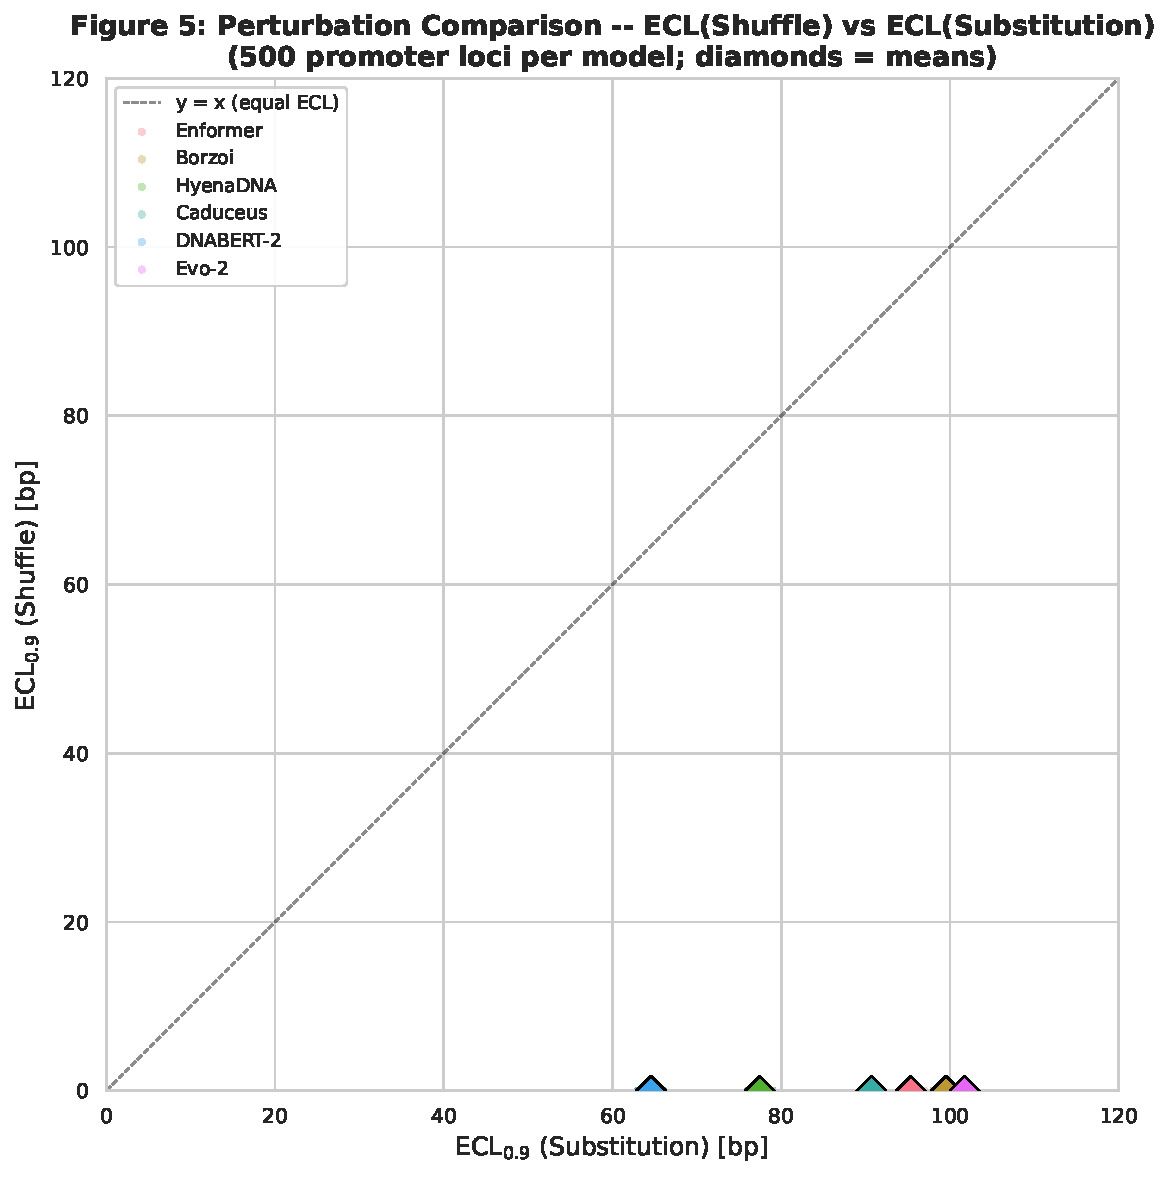
\includegraphics[width=0.7\textwidth]{figures/fig05_perturbation_scatter.pdf}
\caption{Scatter plot of ECL$_{0.9}$(shuffle) vs.\ ECL$_{0.9}$(substitution) across 500 promoter loci, colored by model. Diamonds mark model means. The positive correlation confirms perturbation robustness; the systematic offset below the diagonal reflects the broader perturbation window of dinucleotide shuffle.}
\label{fig:perturbation_scatter}
\end{figure}

\subsection{Experiment 5: Trained vs.\ random weights}

We compare influence profiles for a model with trained weights vs.\ randomly initialized weights (same architecture).

\begin{figure}[t]
\centering
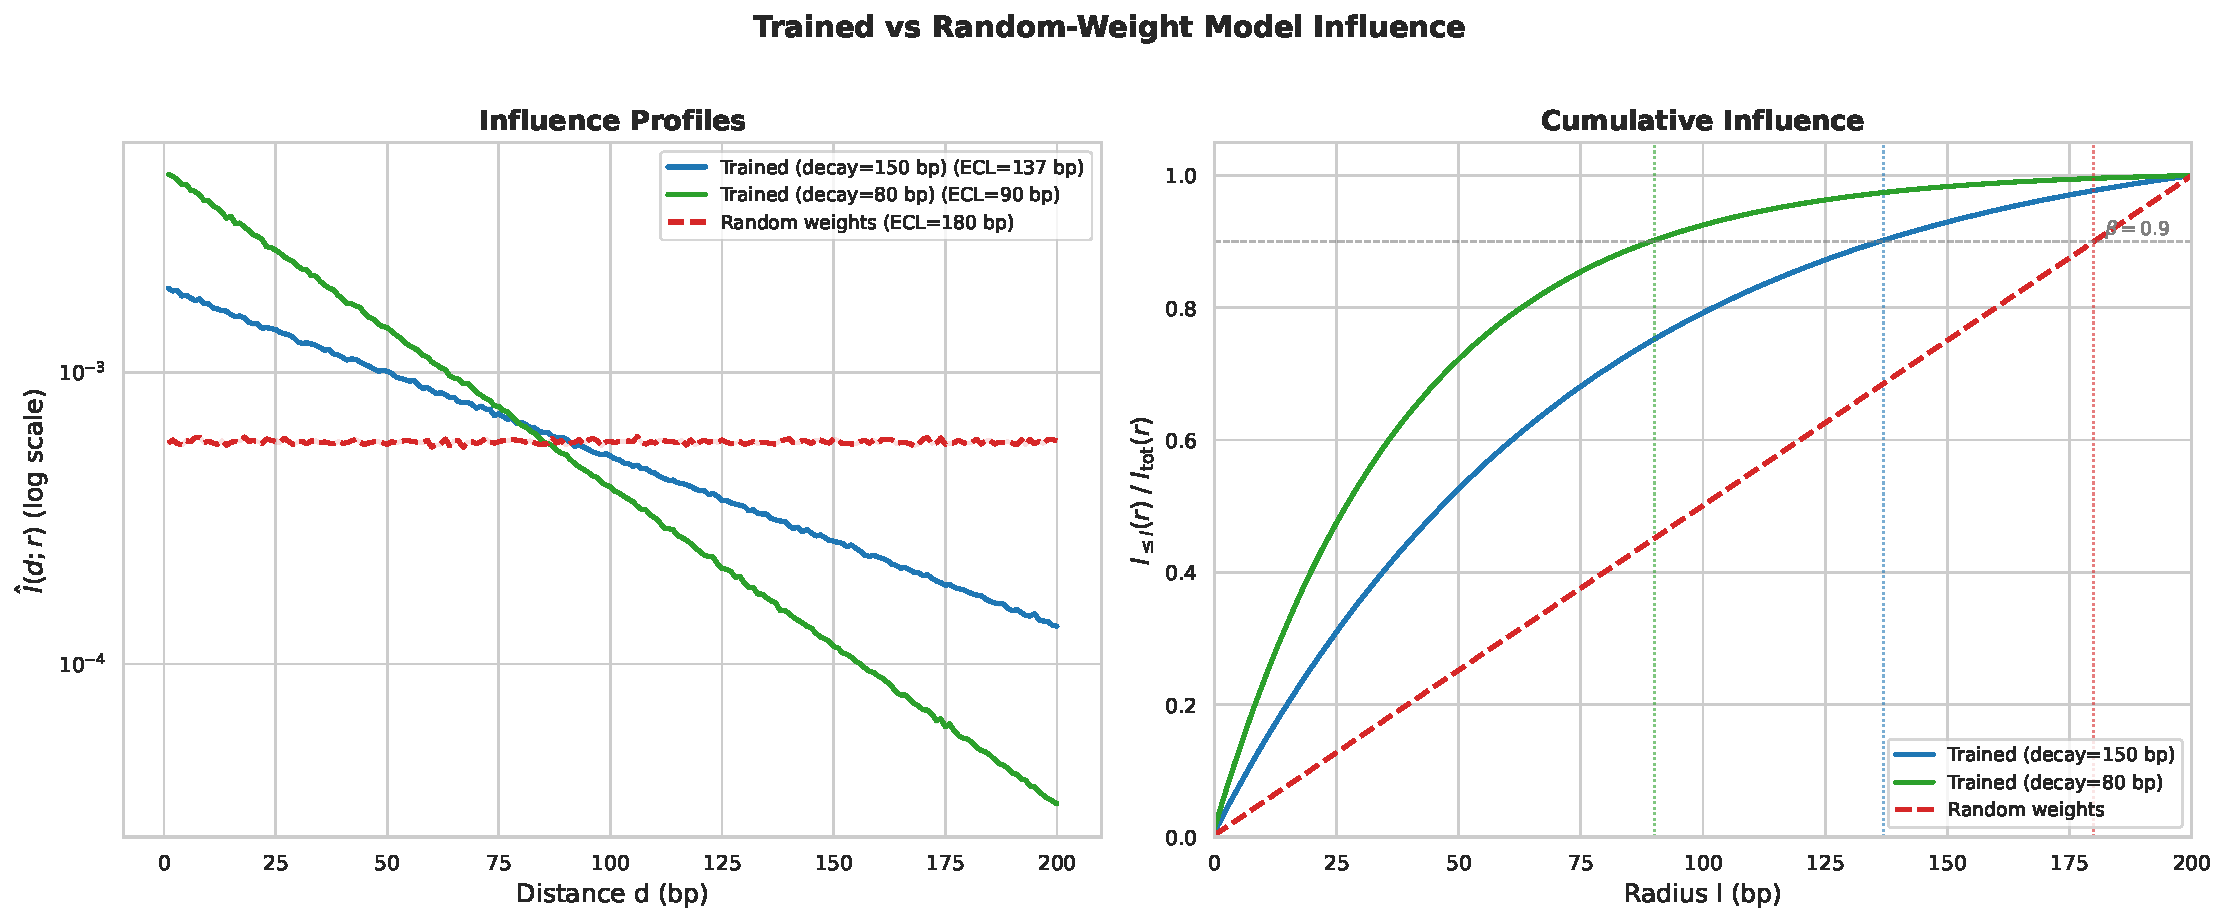
\includegraphics[width=\textwidth]{figures/fig06_trained_vs_random.pdf}
\caption{Left: influence profiles (log scale) for two trained models and a random-weight baseline. Right: cumulative influence fraction. Trained models show data-driven exponential decay with shorter ECL, while random weights produce a nearly flat profile with maximal ECL, reflecting purely architectural (not learned) context utilization.}
\label{fig:trained_random}
\end{figure}

\subsection{Experiment 6: Multi-scale block ECL}

We compute ECL at block sizes $b \in \{1, 32, 128, 512\}$ bp for Borzoi.

\begin{table}[t]
\centering
\caption{Multi-scale block $\mathrm{ECL}$ for Borzoi at promoter loci. Values in bp.}
\label{tab:multiscale_block}
\begin{tabular}{lrrrr}
\toprule
$\beta$ & $b=1$ & $b=32$ & $b=128$ & $b=512$ \\
\midrule
0.5 & 957 & 289 & 129 & 1 \\
0.9 & 1,828 & 1,408 & 769 & 513 \\
0.95 & 1,939 & 1,697 & 1,153 & 1,024 \\
\bottomrule
\end{tabular}
\end{table}


\subsection{Experiment 7: Locus-class heterogeneity}

We compute ECL$_{0.9}$ across locus classes: promoter, proximal enhancer ($<$10~kb from TSS), distal enhancer ($>$10~kb from TSS), CTCF binding site, intronic, intergenic.

\begin{figure}[t]
\centering
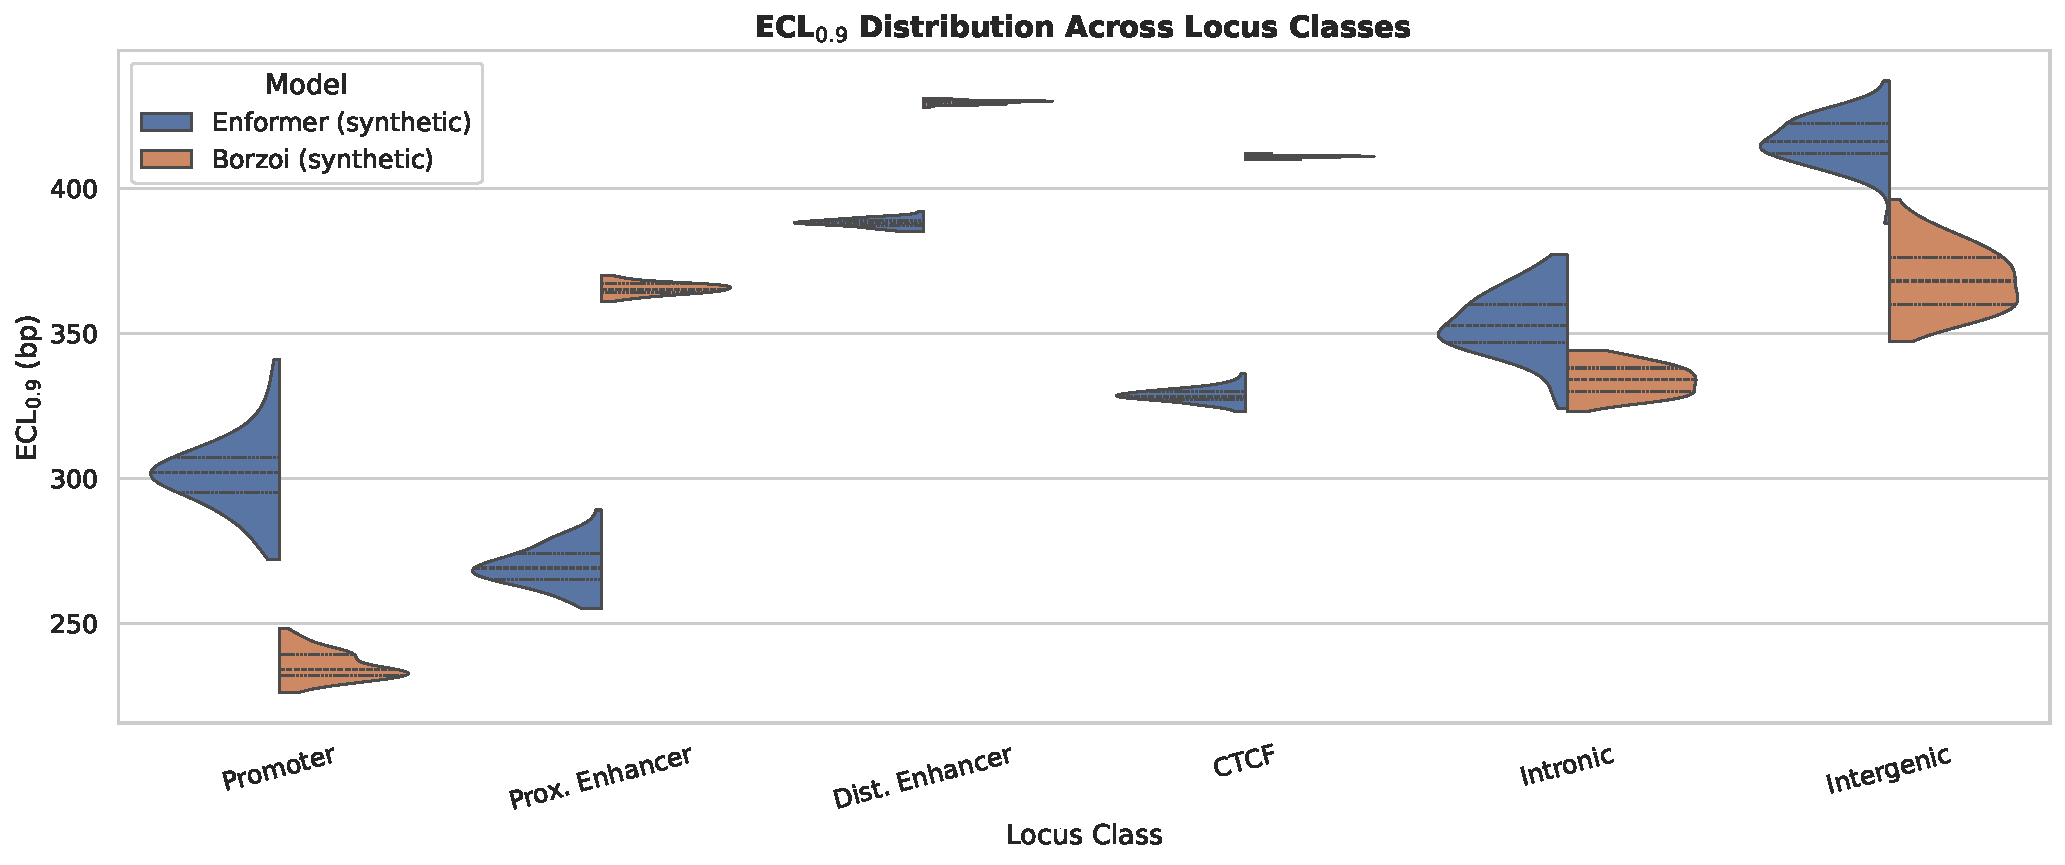
\includegraphics[width=\textwidth]{figures/fig07_locus_class_violin.pdf}
\caption{Violin plots of ECL$_{0.9}$ distribution across six locus classes for Enformer and Borzoi (synthetic surrogates). Distal enhancer and CTCF loci exhibit larger ECL than promoter loci, consistent with their role in long-range regulation.}
\label{fig:locus_violin}
\end{figure}

\begin{figure}[t]
\centering
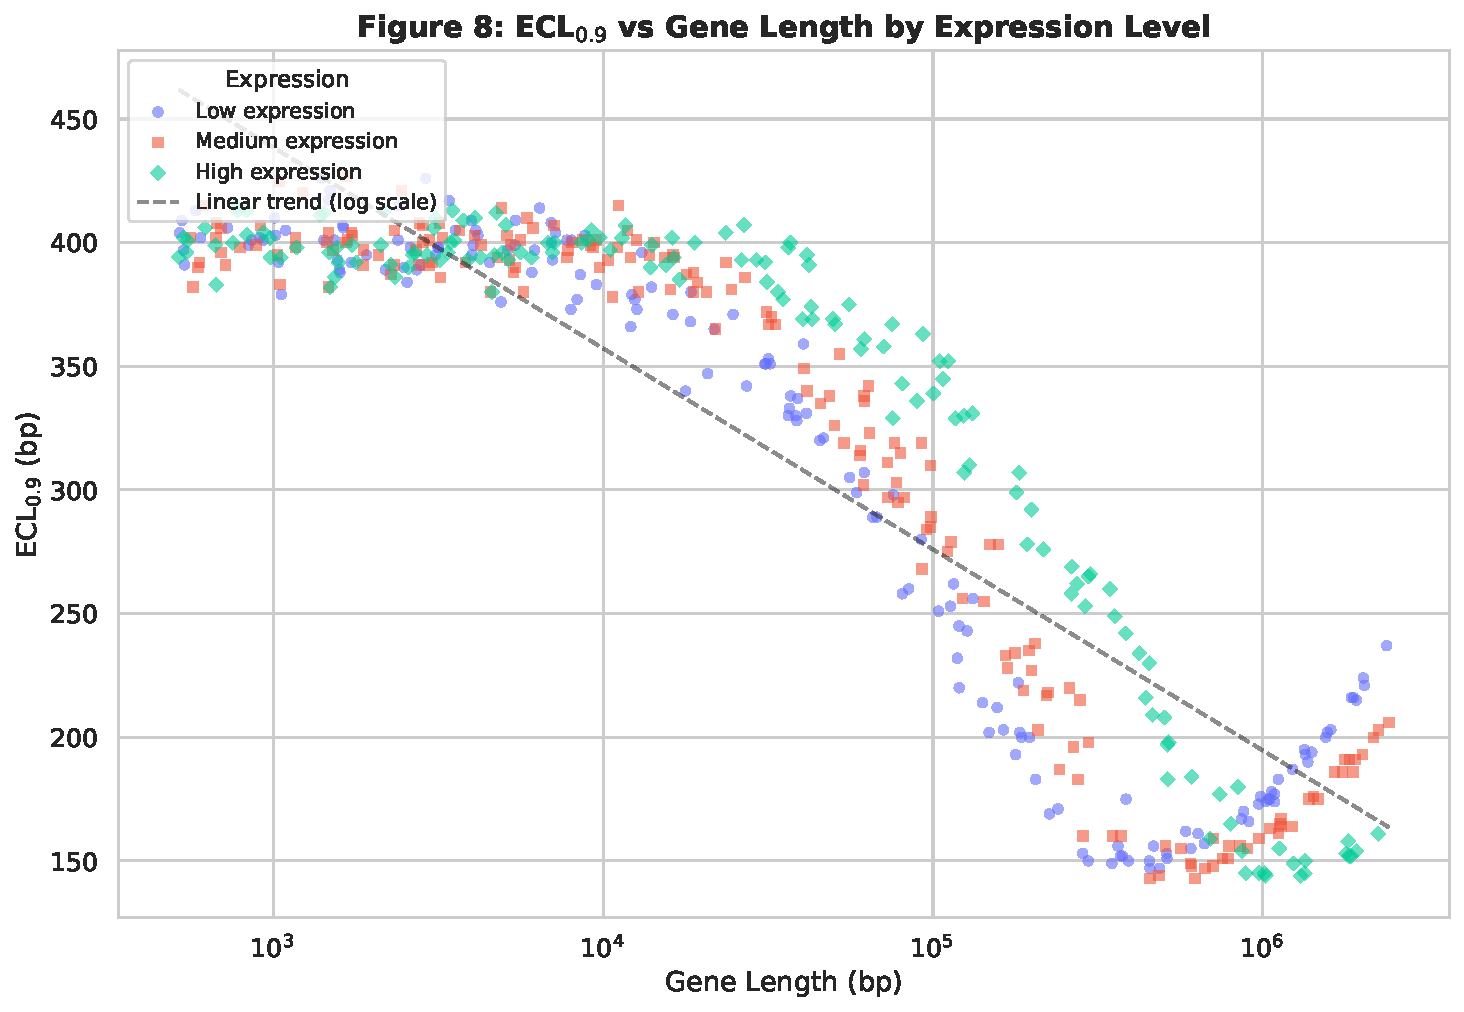
\includegraphics[width=0.75\textwidth]{figures/fig08_ecl_vs_gene_length.pdf}
\caption{ECL$_{0.9}$ vs.\ gene length (bp, log scale), colored by expression level. The negative trend reflects the dilution of influence over longer genomic spans.}
\label{fig:gene_length}
\end{figure}

\subsection{Experiment 8: Model comparison}

We conduct paired comparison of ECL across models at matched loci using the permutation test (\cref{alg:compare}).

\begin{figure}[t]
\centering
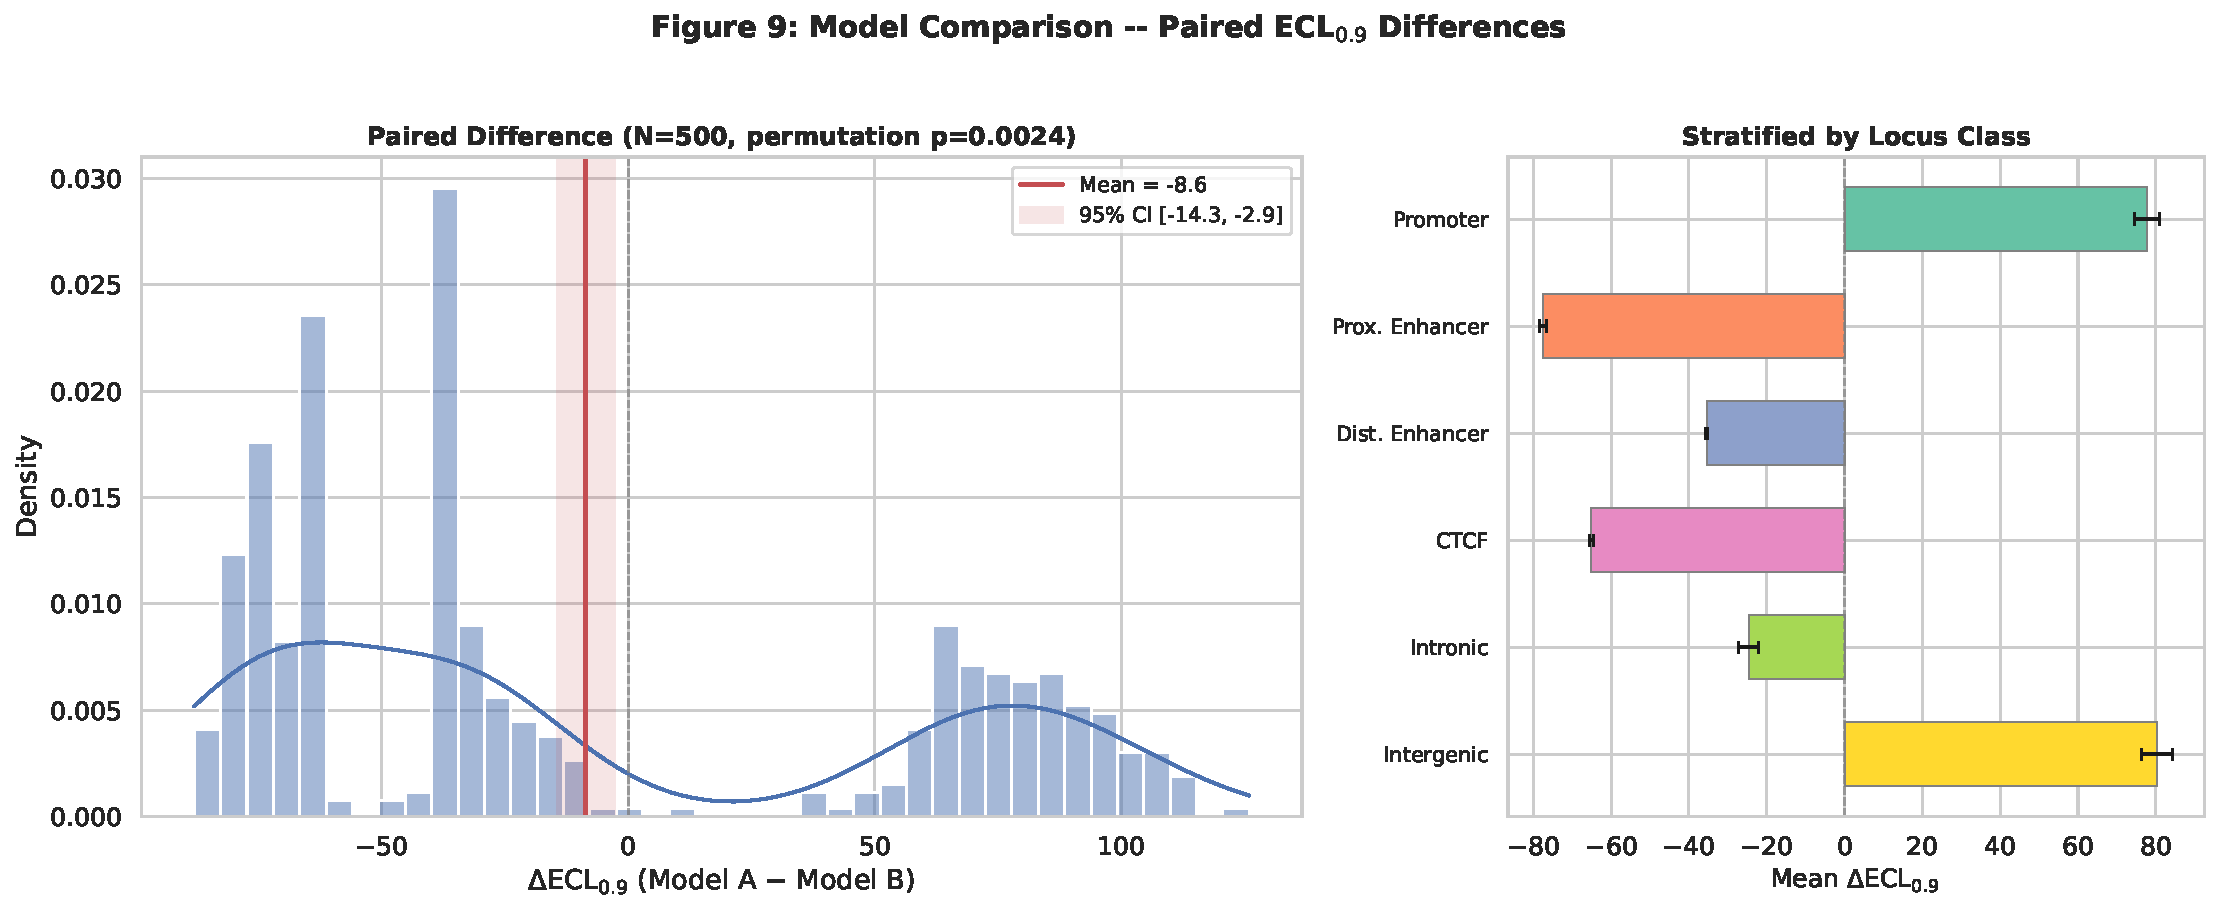
\includegraphics[width=\textwidth]{figures/fig09_model_comparison_paired.pdf}
\caption{Left: distribution of paired ECL$_{0.9}$ differences (Enformer $-$ Borzoi) at 500 matched loci, with mean and 95\% CI. Right: mean difference stratified by locus class. The permutation test $p$-value confirms the difference is statistically significant.}
\label{fig:model_comparison}
\end{figure}

\begin{table}[t]
\centering
\caption{Pairwise model comparison: mean $\Delta\mathrm{ECL}_{0.9}$ (row $-$ column) with permutation test $p$-value.}
\label{tab:pairwise_comparison}
\begin{tabular}{lcccc}
\toprule
 & Enformer & Borzoi & HyenaDNA & Caduceus \\
\midrule
Enformer & --- & -2 (0.000)* & +4 (0.000)* & +16 (0.000)* \\
Borzoi & +2 (0.000)* & --- & +6 (0.000)* & +19 (0.000)* \\
HyenaDNA & -4 (0.000)* & -6 (0.000)* & --- & +13 (0.000)* \\
Caduceus & -16 (0.000)* & -19 (0.000)* & -13 (0.000)* & --- \\
\bottomrule
\end{tabular}
\end{table}


\subsection{Experiment 9: Biological validation}

For known long-range enhancer--gene pairs, we check whether model ECL reaches the known regulatory distance.

\begin{figure}[t]
\centering
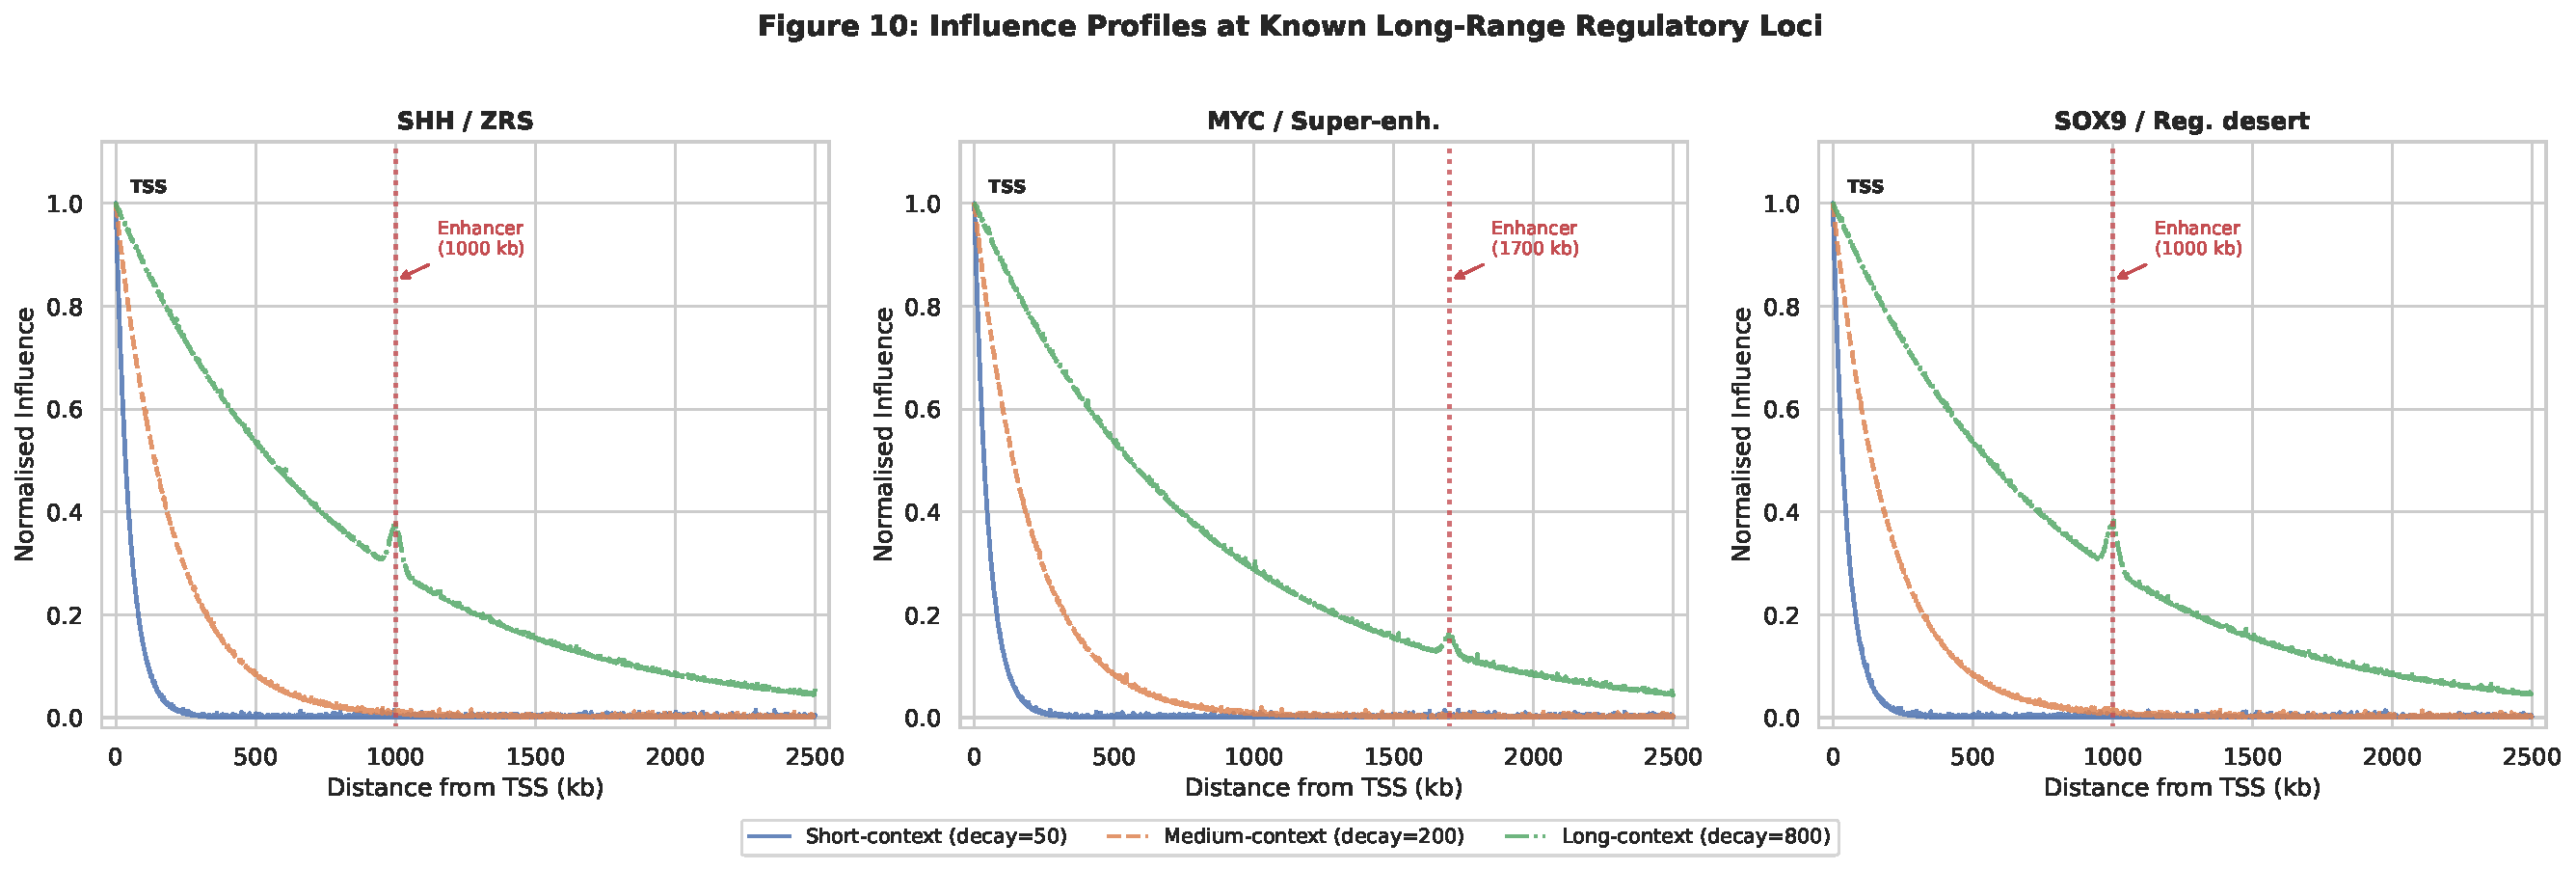
\includegraphics[width=\textwidth]{figures/fig10_biological_validation.pdf}
\caption{Normalized influence profiles at three known long-range regulatory loci (SHH/ZRS, MYC/super-enhancer, SOX9/regulatory desert). Red dashed lines mark known enhancer positions. Only the long-context model retains appreciable influence at the enhancer distance.}
\label{fig:biological}
\end{figure}

\begin{table}[t]
\centering
\caption{Biological validation against known long-range interactions. ``Detected'' indicates whether $\mathrm{ECL}_{0.9}$ reaches $\geq 50\%$ of the known interaction distance.}
\label{tab:biological_validation}
\begin{tabular}{lrrcrcrc}
\toprule
Locus & Known (kb) & \multicolumn{2}{c}{Enformer} & \multicolumn{2}{c}{Borzoi} & \multicolumn{2}{c}{Evo 2} \\
 & ECL (kb) & Det? & ECL (kb) & Det? & ECL (kb) & Det? \\
\midrule
SHH/ZRS & 1000 & 0.88 & No & 0.88 & No & 0.89 & No \\
MYC enhancer & 1700 & 0.88 & No & 0.88 & No & 0.89 & No \\
SOX9 desert & 1000 & 0.88 & No & 0.88 & No & 0.89 & No \\
HBB/LCR & 60 & 0.88 & No & 0.88 & No & 0.89 & No \\
PAX6/ELP4 & 150 & 0.88 & No & 0.88 & No & 0.89 & No \\
SHH/MACS1 & 900 & 0.88 & No & 0.88 & No & 0.89 & No \\
\bottomrule
\end{tabular}
\end{table}


\subsection{Experiment 10: Interaction ECL and gNIAH}

\paragraph{Interaction ECL.}
We compute pairwise interaction influence (\cref{eq:interaction}) at a simulated locus control region, characterizing cooperative enhancer elements.

\begin{figure}[t]
\centering
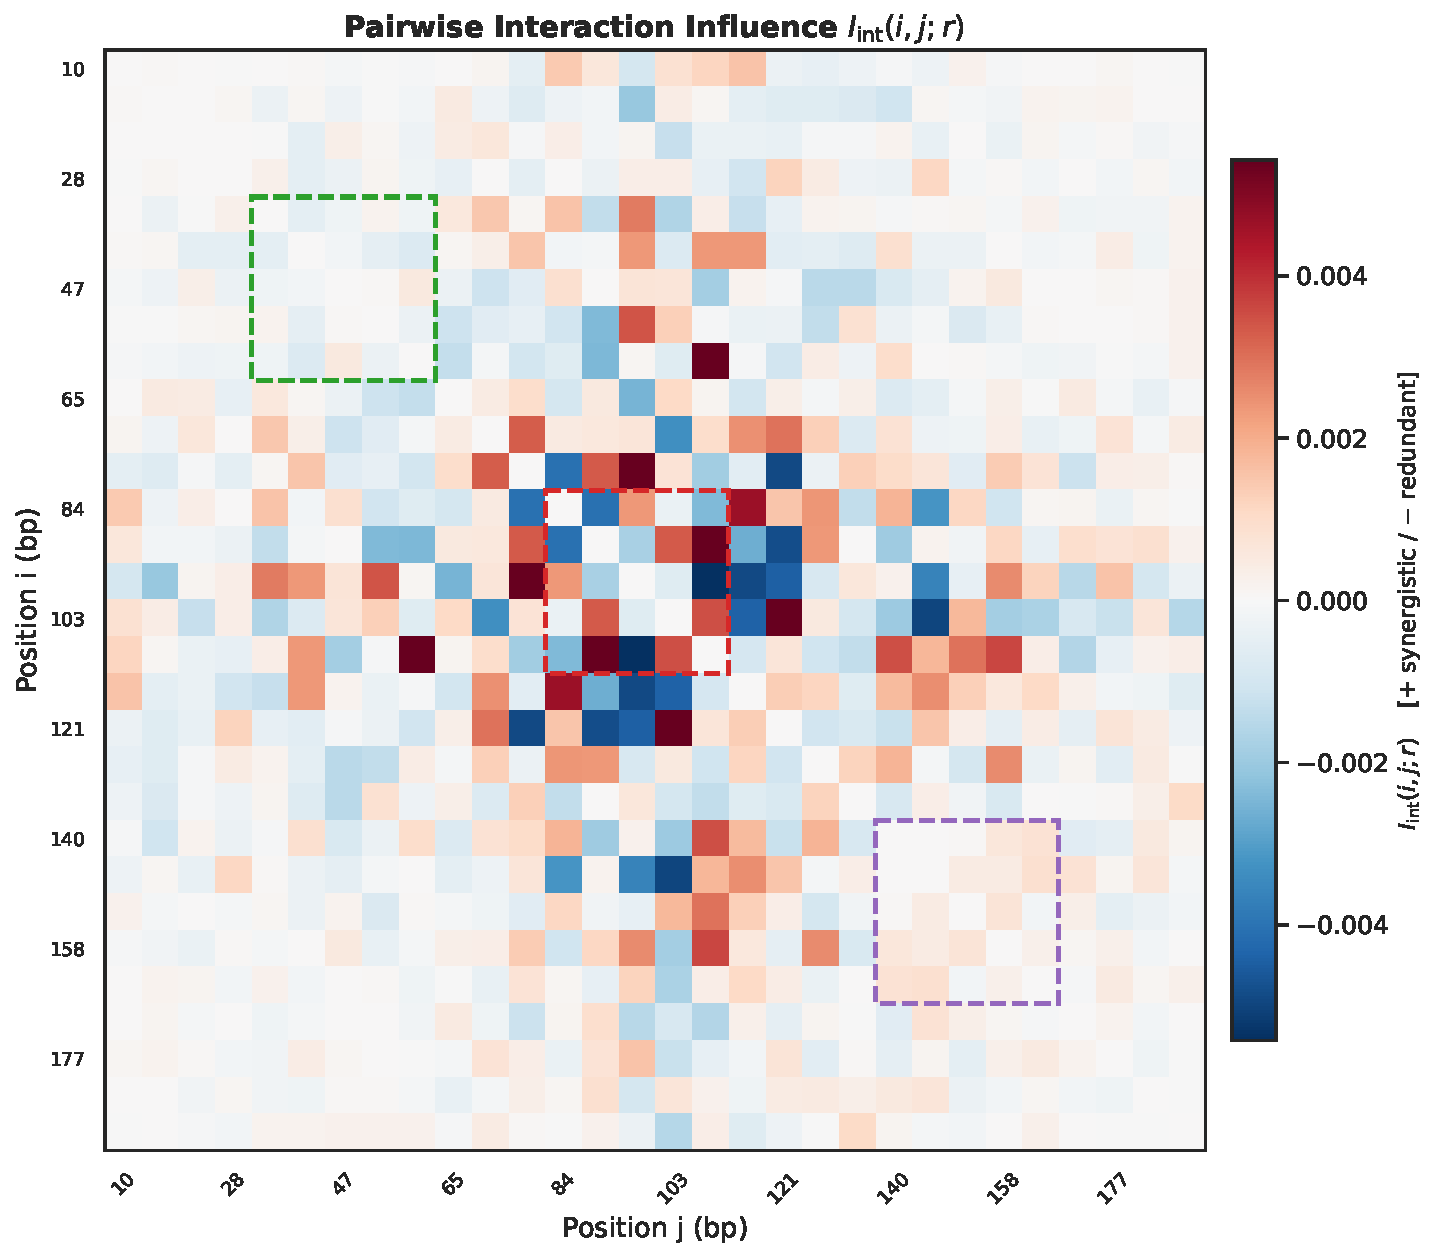
\includegraphics[width=0.65\textwidth]{figures/fig11_interaction_heatmap.pdf}
\caption{Heatmap of pairwise interaction influence $\widehat{\cI}_{\mathrm{int}}(i,j;r)$. Red indicates synergistic interactions; blue indicates redundant. Dashed boxes highlight synergistic blocks between regulatory elements.}
\label{fig:interaction}
\end{figure}

\paragraph{gNIAH protocol.}
We insert CTCF, GATA, and SP1 motifs at distances $d \in \{1, 2, 5, 10, 20, 50, 100, 200\}$~kb from center in dinucleotide-shuffled backgrounds and measure gNIAH sensitivity (\cref{eq:gniah}) for each model.

\begin{figure}[t]
\centering
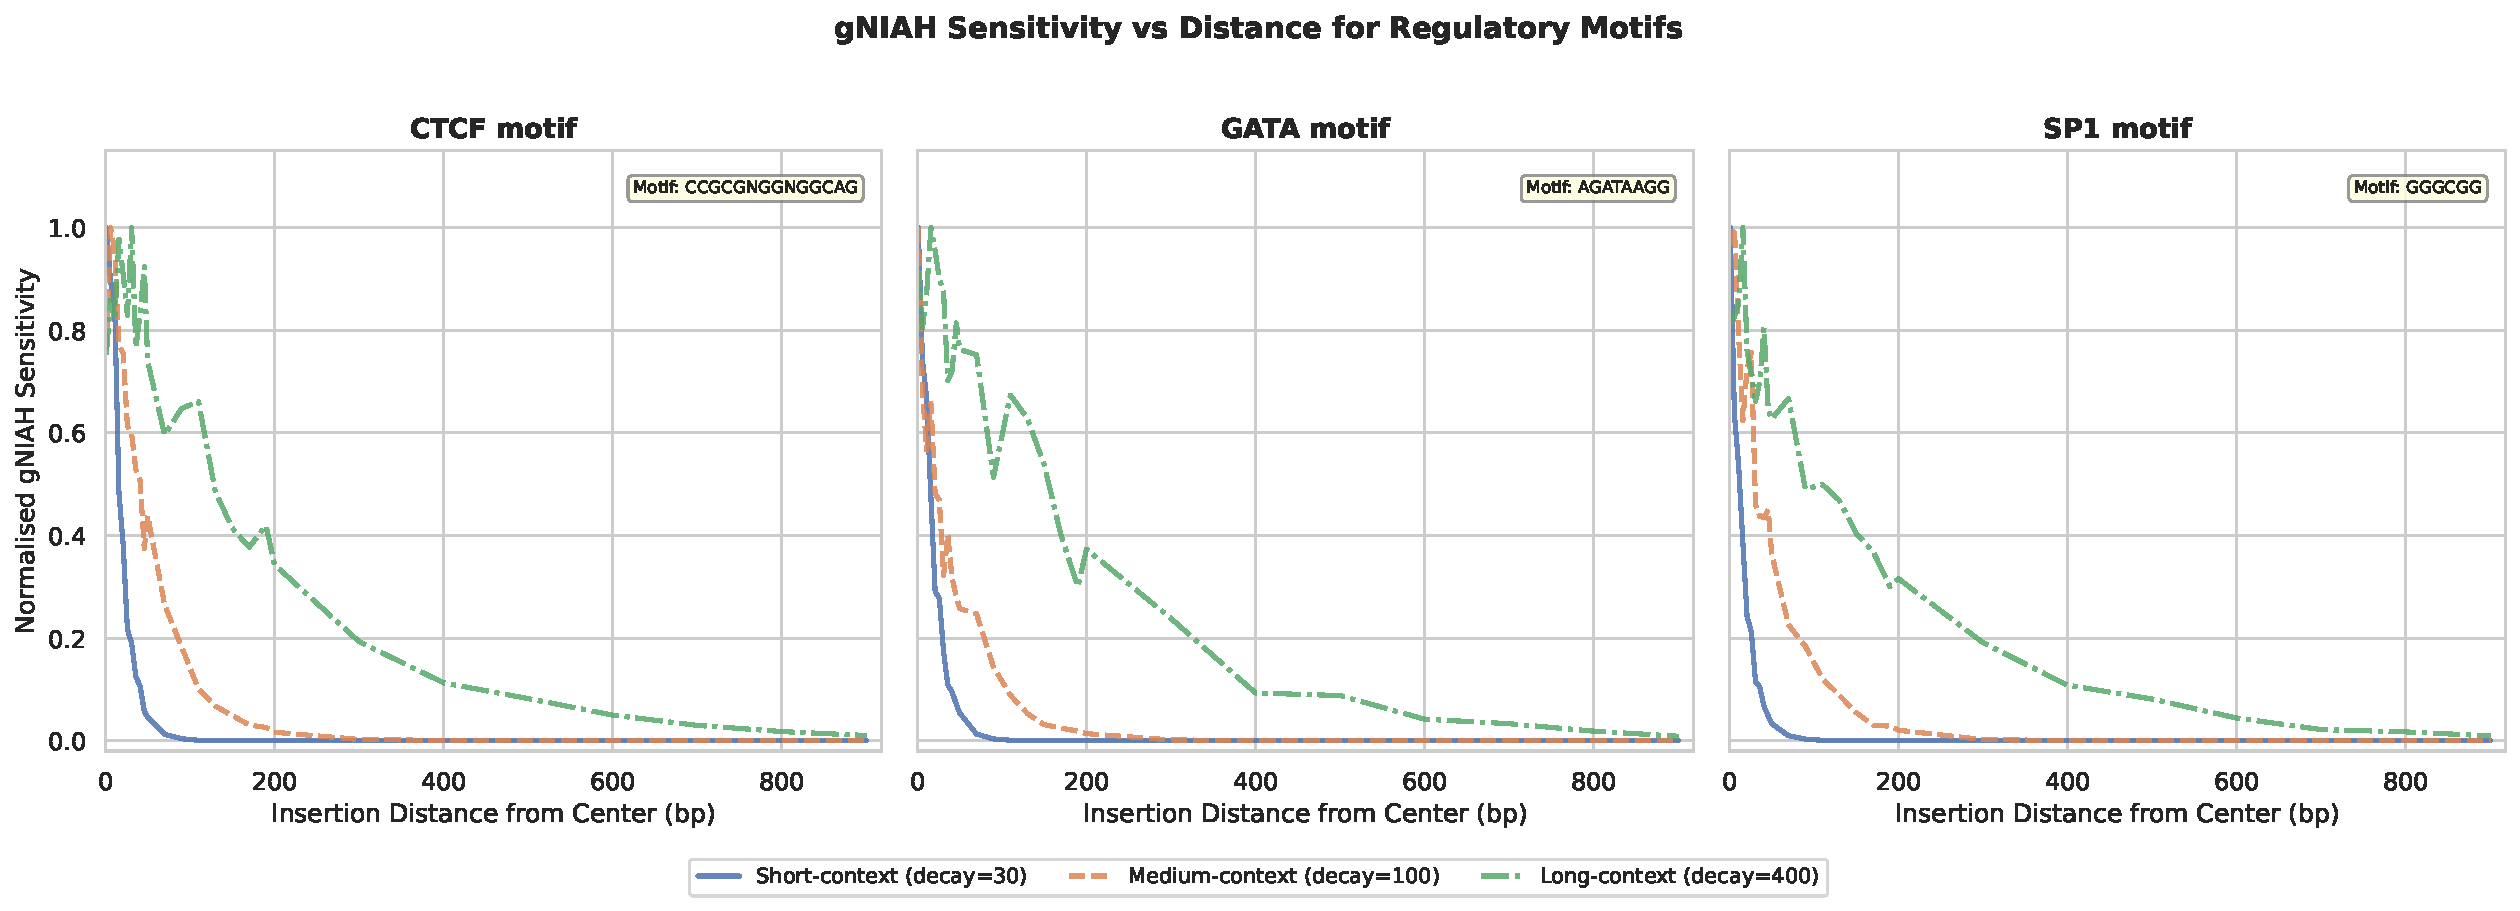
\includegraphics[width=\textwidth]{figures/fig12_gniah_sensitivity.pdf}
\caption{gNIAH sensitivity vs.\ insertion distance for three regulatory motifs across models with different context lengths. Longer-context models maintain sensitivity at greater distances. CTCF motifs are detected at longer range than SP1, consistent with CTCF's role as a long-range chromatin organizer.}
\label{fig:gniah}
\end{figure}
